\begin{frame}{$d(K^-, n)$ reaction kinematics}
  \begin{tabular}{cc}
    \begin{minipage}{0.4\hsize}
      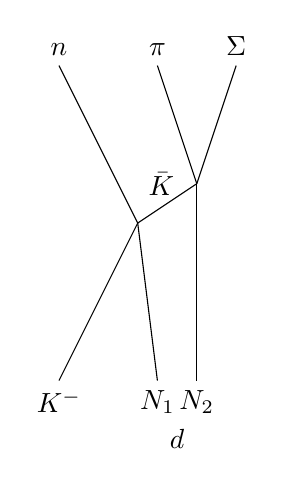
\begin{tikzpicture}
        \draw (-1.0, -2.0) node [ below ] {$K^-$} -- (0.0, 0.0);
        \draw ( 0.5, -2.5) node [ below ] {$d$};
        \draw ( 0.25, -2.0) node [ below ] {$N_1$} -- (0.0, 0.0);
        \draw ( 0.75, -2.0) node [ below ] {$N_2$} -- (0.75, 0.5);

        \draw (0.0, 0.0) -- (-1.0, 2.0) node [ above ] {$n$};

        \draw (0.3, 0.5) node {$\bar{K}$};
        \draw (0.0, 0.0) -- (0.75, 0.5);
        
        \draw (0.75, 0.5) -- (0.25, 2.0) node [ above ] {$\pi$};
        \draw (0.75, 0.5) -- (1.25, 2.0) node [ above ] {$\Sigma$};
      \end{tikzpicture}
    \end{minipage}
    \begin{minipage}{0.6\hsize}
    \end{minipage}
  \end{tabular}
\end{frame}
